
\chapter{Pipeline Assembly in Python}
\label{chap:pipeline}
This chapter serves as a link between the preceding three chapters, illustrating the process of assembling the different components into a functional pipeline.
While providing a comprehensive explanation of the pipeline is considered unnecessary for the thesis, the focus is placed on highlighting the crucial components and design choices.
The complete source code is available upon request.

\section{Approach to Concurrency}
As discussed in \todo using \gls{asyncio} is significantly more performant than using threads.


\begin{figure}
    \centering
    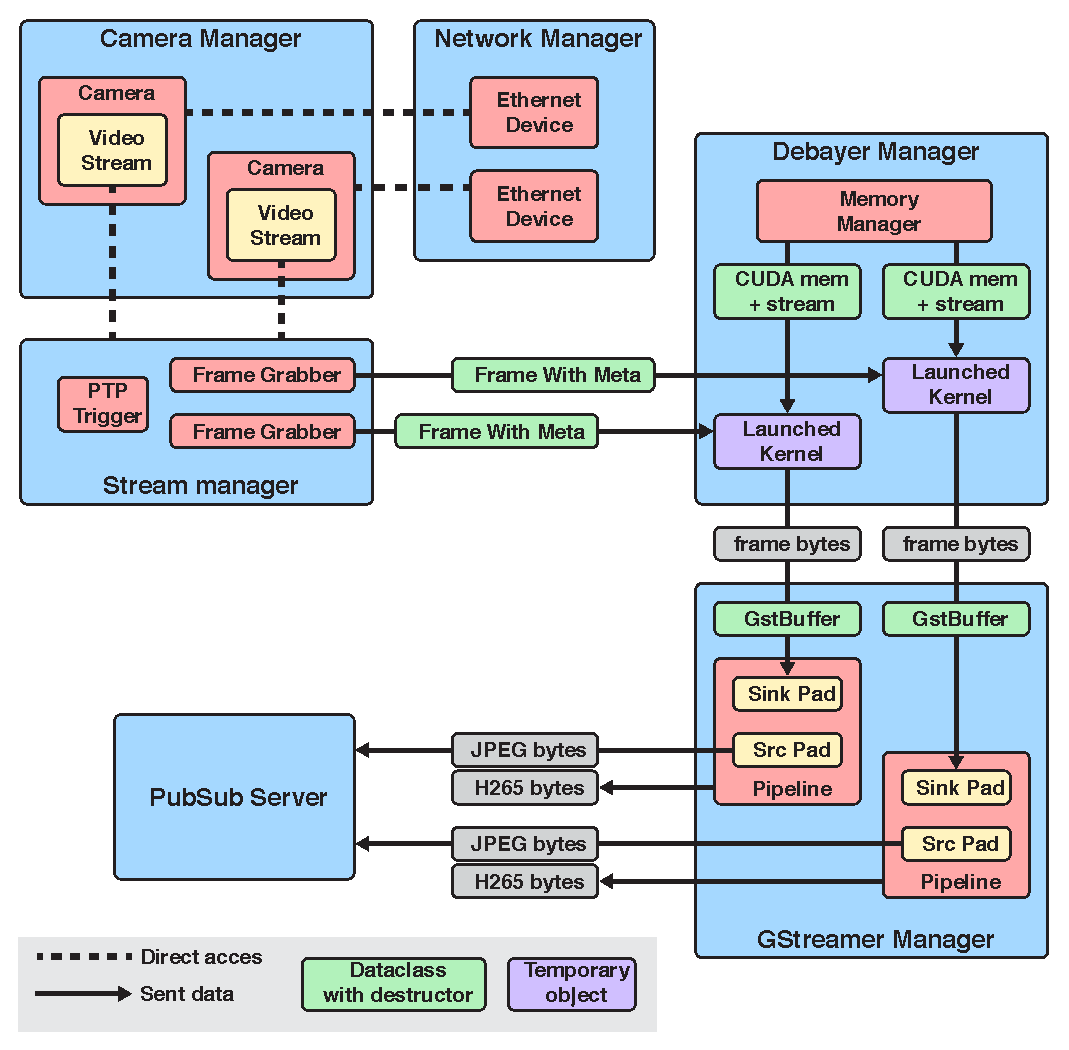
\includegraphics[width=\textwidth]{figures/object_overview.pdf}
    \caption{Class diagram showing the relationship between the classes in the pipeline and how thei interact.}
    \label{fig:pipeline_current}
\end{figure}

\subsection{Sharing Subcomponents}
Two sets elements in the pipeline are created and owned and destroyed by one object but used direcly by another.
This is done to solve synchronization problems during creaton, configuration and utilization of the objects.

The ethernet device objects are created, owned and configured by the Network Manager, and used by directly by the Camera Manager during the creation of each Camera object.
The network manger ensures that they never are configured to have overlapping subnets, as this causes issues during the discovery, creation and operation of the cameras.

The Video Stream objects are created and confibured by their corresponding camera object and used direcly by the Video Stream Manager, which grabs frames and makes sure that left and right frames are synchronized.

\subsection{Graceful Shutdown}
In real-time systems involving external hardware, it is essential to implement controlled shutdown procedures to avoid potential complications and issues in future runs.

On the \sr it is especially important to handle the camera and stream objects appropriately to avoid the cameras becoming inaccessible.
This is achieved by utilizing the \code{with} and \code{async with} syntax in Python, along with \code{try-finally} blocks, to ensure proper resource cleanup.

In case the cameras become inaccessible, a possible solution is to temporarily disable the Ethernet interface they are connected to for approximately two minutes.
This action appear to trigger an internal reset of the cameras, restoring their functionality.

\subsection{Custom Destructors}
Several custom message types have been developed with custom destructors to ensure proper cleanup.

The Frame With Meta object contains the data and relevant metadata for a single frame.
The underlying memory is managed internally by \gls{arena-api} and needs to be explicitly freed back to the underlying memory pool in order for new frames to be allocated.
This object has a custon \code{free} function used to free the underlying memory and \code{__del__} function that logs a warning if the memory has not been freed explicitly and frees it.

Allocating\gls{cuda} memory is a slow operation.
According to \gls{nsys}, allocating the tecessary memory to perform the transformation presented in Chapter \ref{chap:debayer} takes more time than the transformation itself.
To avoid this overhead a custom\gls{cuda} memory pool was implemented that r\gls{cuda} CUDA memory in order to avoid allocating and freeing memory and stream objects for each frame.
This pool is managed by the Memory Manager.
When the\gls{cuda} Memor\gls{cuda} CUDA Stream used by a kernel goes out of scope

Finally, Gstreamer uses their own garbage collecion system and reference counting to manage memory.
Fortunately the \gls{pygo} bindings for Gstreamer handles this automatically by having the python object participate in the reference counting, ensuring that the underlying Gstreamer object is not freed before the \py object is.


\subsection{Debayer Manager}
The main role of the debayer manager is to integrate the\gls{cuda} code with \py.
To acheive this \gls{pybind11} was used.
\gls{pybind11} is a \gls{cpp} library that allows for the creation of \py bindings for \gls{cpp}, also \gls{cpp} funcions that launch \gls{cuda} kernels.

Several ways are available to pass data between \gls{cpp} and \py, but when working with \gls{cuda} the easiest way is to pass pointers to \gls{numpy} or \gls{cupy} arrays, which are available trough the \code{__array_interface__} and \code{__cuda_array_interface__} respectively \cite{numpyArrayInterfaceProtocol} \cite{cupyInteroperabilityCuPy12}.
It is also possible to pass data as \gls{eigen}.

When working with \gls{pybind11} it is easiets to mamage the memory in \py and pass references to the \gls{cpp} code.

It is worth mentioning that it is also possible to write \gls{cuda} kernels in \py directly through \gls{cupy} as well as other \gls{gpu} accelerated libraries such as \gls{numba} and \gls{pytorch}
Based on prioer experience however these are impossible to debug and should be avoided for anything but the simplest of tasks.